\subsection{Flux}

As propostas citadas necessitavam ser demonstradas em alguma plataforma LIMS que implementa BPMs como base de metodologia na construção de fluxos de trabalho. Com isso, escolhemos o Flux por causa de sua maleabilidade na criação de workflows e a utilização no passado da plataforma.

O Flux é um meta LIMS: ele é capaz de, a partir de um BPM, implementá-lo em forma de fluxo de trabalho dentro do software, com um sistema de permissão robusto para dar aos usuários segurança de dados, além de diminuir o número de dados na tela que pode confundir que está o utilizando.

O Workflow construído no Flux tem um formato de árvore: Uma atividade inicial, sendo uma atividade uma regra de negócio do BPM. Após a atividade inicial ser criada, é criada juntamente a ela uma instância, que separa diferentes processos do mesmo tipo um dos outros.

Como exemplo, temos o cadastro de um paciente em um hospital. Se o cadastro for a primeira atividade do workflow, para dez pacientes a serem cadastrados, 10 instâncias serão criadas, uma para cada cadastro.

Dentro das atividades temos atributos: Valores que podem ser preenchidos para descrever a atividade em questão. Voltando ao exemplo de cadastro de paciente, temos como exemplo de atributos dentro da atividade de cadastro o nome do paciente, data de nascimento, endereço, comorbidades, entre muitos outros que podem pertencer a esta atividade.

Cada atividade pode ter atividades filhas, montando um fluxo de trabalho que podemos ver na imagem \ref{fig:estrutura_workflow}. Com isso, podemos construir um BPM seguindo as regras de negócio da empresa e implementar a funcionalidade da empresa escolhida.

\begin{figure}
    \centering
    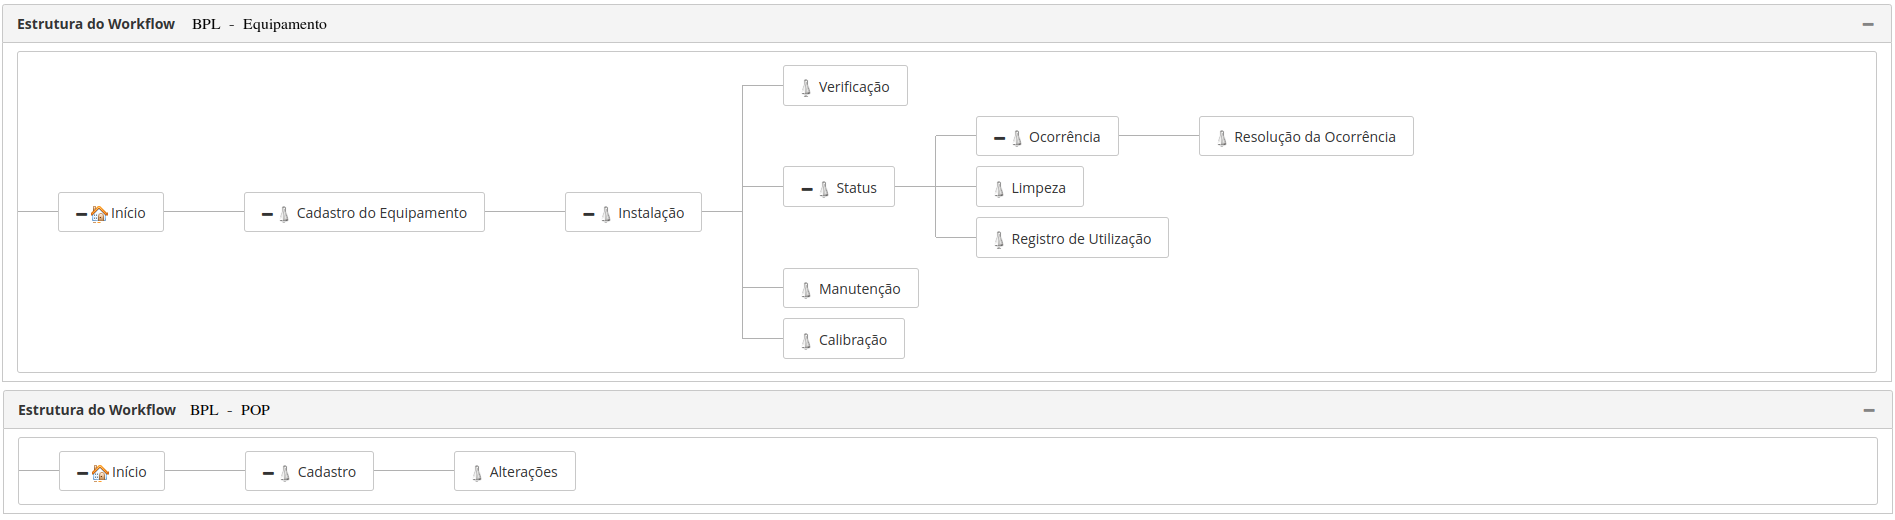
\includegraphics[width=1\textwidth]{imgs/BPL/estrutura.png}
    \caption{Estrutura de dois workflows: BPL - POP e BPL Equipamentos. A atividade inicial destes workflows são as atividades "Cadastro" e "Cadastro do equipamento", respectivamente.}
    \label{fig:estrutura_workflow}
\end{figure}

A estrutura do workflow, as atividades e atributos dela podem ser todos construídos dentro do próprio software, facilitando a implementação destes no ambiente de trabalho, sem que seja necessário o conhecimento de programação.

Existe a possibilidade de adicionar atributos estendidos para cada tipo de objeto, seja um atributo, seja atividade, instância ou até mesmo o próprio workflow.

Ao criar os atributos, podemos especificar o tipo do atributo, seja um número, seja decimal, CPF ou um texto normal, como exemplos, para que seja facilitado o processo de análise dos dados que são cadastrados para cada pessoa.

 \subsubsection{Alterações feitas para workflows dinâmicos}

AS alterações feitas no software para que o workflow dinâmico pudesse ser implementadas foram as de criar uma instância auxiliar que contivesse todas as atividades já contidas na própria atividade, mas com uma atividade inicial diferente da original.

Para selecionar qual atividade inicial será utilizada na visualização atual, também foi alterada a interface para adicionar um seletor. Nele, temos o nome de todas as atividades do workflow selecionado que o usuário tem a permissão de visualizar.

Caso o usuário não selecione nenhuma atividade, a atividade inicial utilizada será a padrão, deixando o workflow na visualização padrão.

\textbf{Imagem do seletor aqui.}

Quando muda-se a estrutura do workflow, devemos ter cuidado com as informações anteriores que existiam e deixa-las disponíveis para acesso, já que o usuário pode querer vê-las durante a execução de outras atividades.

Como exemplo, temos o cadastro de paciente na primeira atividade novamente. Caso o paciente for fazer uma cirurgia, que pode ser uma atividade mais profunda no workflow, devemos ter os dados do paciente disponíveis para o médico que irá realizar aquela atividade.

\subsubsection{Como funciona}

Quando o usuário seleciona a atividade desejada para ser a atividade inicial, a árvore de atividades é reajustada para que a atividade selecionada seja o foco principal da instância.

Para isso, gira-se a árvore de atividades para a direita, tendo todas as atividades anteriores como atividades filhas da selecionada, mantendo a sub árvore de atividades originais intacta.

As atividades anteriores continuam na árvore para que qualquer informação anterior que seja necessária para a execução de atividades posteriores fiquem disponíveis para serem visualizadas e utilizadas pelo usuário.

\begin{figure}
    \centering
    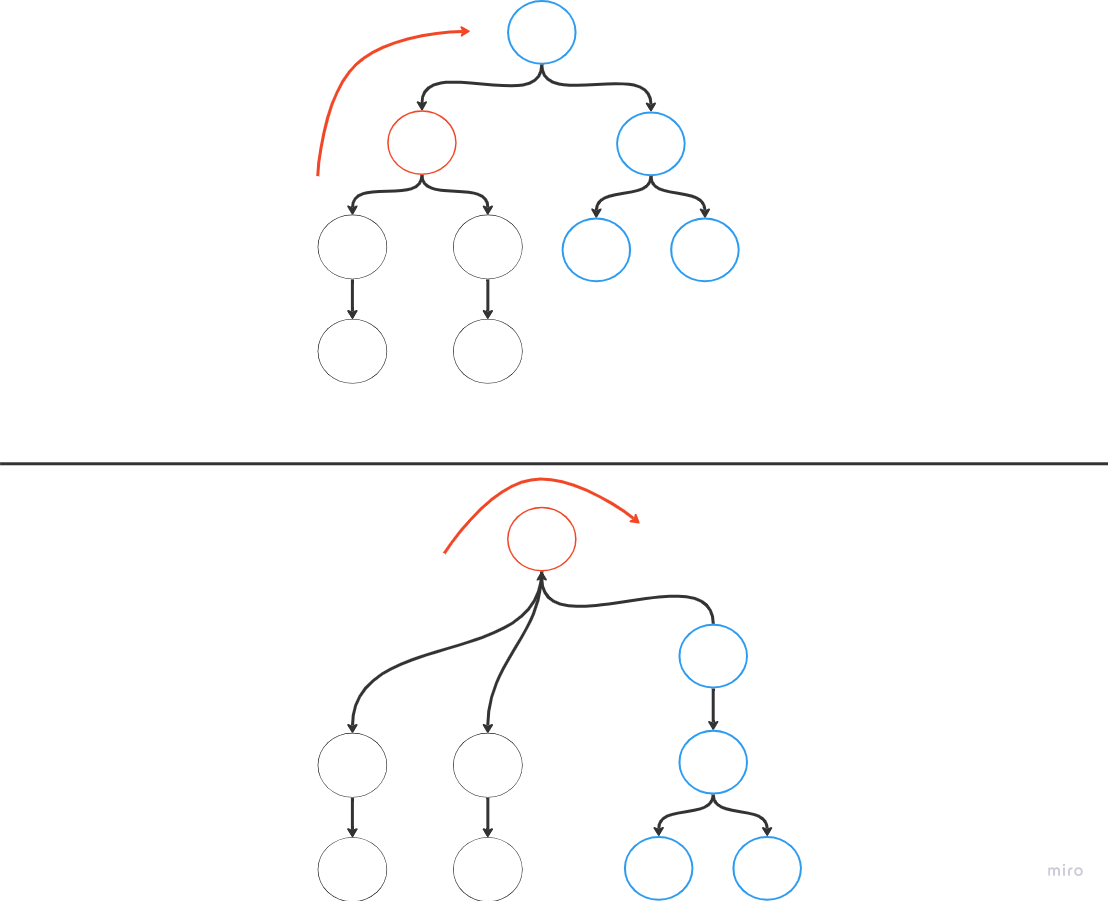
\includegraphics[width=1\textwidth]{imgs/Implementacoes/primeiraImplementacao.png}
    \caption{Representação da primeira implementação de recursos: Workflows dinâmicos. Na imagem de cima, podemos ver a implementação original de um workflow genérico que está prestes a ser reconstruído. A atividade em vermelho será utilizada como atividade inicial. Com isso, a seta em vermelho representa a alteração feita no workflow.}
    \label{fig:primeira_implementacao}
\end{figure}

No Flux, esta funcionalidade faz com que atividades antigas tenham uma cor diferente na interface do usuário para que seja claro que as atividades vistas pelo usuário são atividades anteriores da atividade selecionada.

\subsection{Alterações feitas para múltiplas atividades iniciais}

BPMs não tem suporte para múltiplas atividades iniciais: Um processo deve iniciar e terminar da mesma forma, passando por todo o fluxo de trabalho da organização. \R
Como um mesmo workflow pode ter troca de informações com alguma parte de outros workflows, foi idealizado uma nova funcionalidade para u workflow: Múltiplas atividades iniciais.

Com múltiplas atividades iniciais, é possível agregar diversos workflows que tratam do mesmo laboratório juntos, e cada usuário escolhe em que parte do workflow ele quer (e pode) iniciar um novo trabalho.

Assim, quando se inicia os trabalhos em uma parte diferente de um workflow, e este workflow se comunica com outro BPM, pode-se fazer uma requisição de informações ou execução de atividade por meio do sistema de permissões.

\subsubsection{Como funciona}

Vamos utilizar o exemplo de um pedido de exame em um workflow médico e o recebimento deste pedido de exame e execução do mesmo.
Um médico cria uma instância de paciente, cadastrando-o e seguindo o fluxo de trabalho comum de atendimento.
O laboratórios do hospital também tem seu próprio workflow, onde são cadastrados equipamentos para análise de amostras.
Antes, os workflows ficariam separados, sem comunicação entre eles.

Com o novo recurso implementada, os workflows podem compartilhar atividades como o pedido de exame: O médico tem a permissão de executar o pedido de exame, mas ele não aprova a atividade, quem irá aprovar a atividade é o técnico de laboratório.

O técnico de laboratório recebe uma notificação que a atividade foi executada e pode aprovar ou reprovar a atividade.
Aprovando a atividade, o técnico continua com seu workflow normalmente até o resultado.
Caso o médico tenha permissão de visualizar as atividades entre o pedido de exame e resultado do exame, o médico poderá ver todo o processo de análise.
Caso contrário, o sistema de permissões controla o que o médico poderá ver, que será o pedido de exame e o resultado do exame.

Assim, a árvore de atividades, caso o médico tenha permissão de visualizar apenas o pedido de exame e a execução, fica da maneira representada na figura \ref{fig:segunda_implementacao}

\begin{figure}
    \centering
    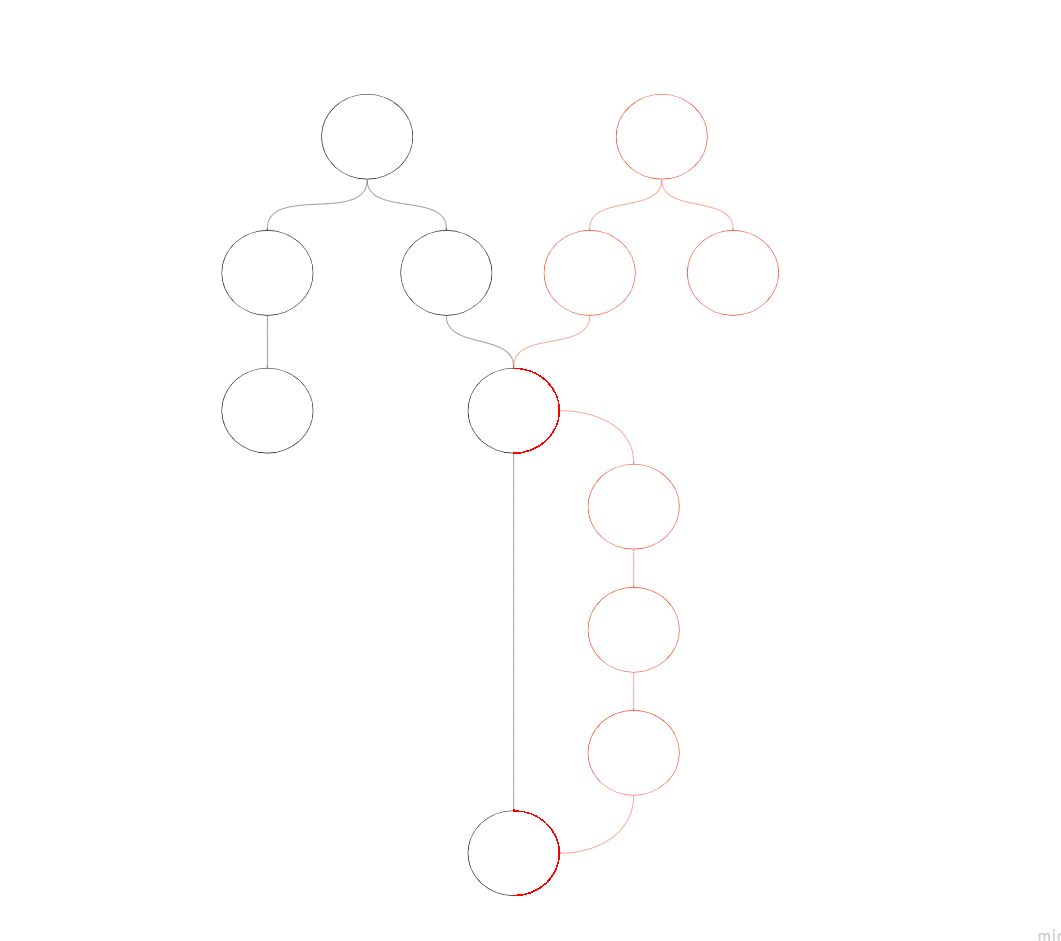
\includegraphics[width=1\textwidth]{imgs/Implementacoes/segundaImplementacao.png}
    \caption{Representação da implementação de múltiplas atividades iniciais. Neste exemplo, temos a instância de pacientes em preto e em vermelho temos o workflow do técnico de laboratório. Podemos ver que as atividades em preto e vermelho são compartilhadas, e apenas o técnico tem permissão de visualização das atividades entre o pedido de exame e o resultado do pedido.}
    \label{fig:segunda_implementacao}
\end{figure}

% Workflow grande feito no Flux